%% Time-stamp: <2018-10-18 20:24:12 (marc)>
\documentclass[xcolor=x11names,compress,mathserif]{beamer}

\newcommand{\hackspace}{\hspace{4.2mm}}
\newcommand{\showstudent}[1]{}
\newcommand\hmmax{0}
\newcommand\bmmax{0}


\usepackage{../includes/MarkMathCmds}





% talk/author information
\newcommand{\authorname}{Mark van der Wilk}
\newcommand{\authoremail}{m.vdwilk@imperial.ac.uk}
\newcommand{\authoraffiliation}{
  Department of Computing\\Imperial
  College London}
\newcommand{\authortwitter}{markvanderwilk}
\newcommand{\slidesettitle}{\imperialBlue{Overfitting \& Generalisation}}
\newcommand{\footertitle}{Overfitting \& Generalisation}
\newcommand{\location}{Imperial College London}
\newcommand{\talkDate}{November 4, 2022}



\date{\imperialGray{\talkDate}}




% load defaults
\selectcolormodel{rgb}
\usepackage{ifxetex,ifluatex}
\newif\ifxetexorluatex
\ifxetex
  \xetexorluatextrue
\else
  \ifluatex
    \xetexorluatextrue
  \else
    \xetexorluatexfalse
  \fi
\fi

\usepackage{textpos}
%\usepackage{arabtex}
\usepackage{tikz}
\usetikzlibrary{decorations.markings}
\usetikzlibrary{arrows}
\usetikzlibrary{shapes}
\usetikzlibrary{plotmarks}
\usetikzlibrary{mindmap,trees,backgrounds}

\tikzstyle{every picture}+=[remember picture]

%\usepackage{movie15}
% \usepackage{pdfpages}
%\usepackage{xmpmulti}

\usepackage{anyfontsize}
\usepackage{wrapfig}
\usepackage{animate}
\usepackage{multirow}
\usepackage{multimedia}
\usepackage{xmpmulti}
%\usepackage[latin9]{inputenc}
\usepackage[english]{babel}
\usepackage{scalefnt}
\usepackage{verbatim}
\usepackage{url}
% \usepackage{pgf,pgfarrows,pgfnodes}
\usepackage{textpos}
\usepackage[tight,ugly]{units}
\usepackage{url}
\usepackage{bbm}
\usepackage[english]{babel}
\usepackage{fancyhdr}
\usepackage{bm} % correct bold symbols, like \bm
\usepackage{amsmath}
\usepackage{amsfonts}
\usepackage{amssymb}
\usepackage{mathrsfs}
\usepackage{mathtools}
\usepackage{color}
\usepackage{cancel}
\usepackage{algorithm}
\usepackage{algpseudocode}
\usepackage{mathrsfs}
\usepackage{listings}
\usepackage{graphicx} % for pdf, bitmapped graphics files
\usepackage{mathtools}
\usepackage{units}
\usepackage{subfig}
\usepackage{enumerate}
\usepackage[comma,authoryear]{natbib}
\usepackage{dsfont}


\ifxetexorluatex
\usepackage{fontspec}
\setmainfont[Scale=0.8]{OpenDyslexic-Regular}
\else
\usefonttheme{professionalfonts}
\fi

\renewcommand{\vec}[1]{{\boldsymbol{{#1}}}} % vector
\newcommand{\mat}[1]{{\boldsymbol{{#1}}}} % matrix
% \newcommand{\KL}[2]{\mathrm{KL}(#1\|#2)} % KL divergence
\newcommand{\R}[0]{\mathds{R}} % real numbers
\newcommand{\Z}[0]{\mathds{Z}} % integers
\newcommand{\tr}[0]{\text{tr}} % trace
% \newcommand{\inv}{^{-1}}
% \DeclareMathOperator*{\diag}{diag}
\newcommand{\E}{\mathds{E}} % expectation
\newcommand{\var}{\mathds{V}}
\newcommand{\gauss}[2]{\mathcal{N}\big(#1,\,#2\big)}
\newcommand{\gaussx}[3]{\mathcal{N}\big(#1\,|\,#2,\,#3\big)}
\newcommand{\gaussBig}[2]{\mathcal{N}\left(#1,\,#2\right)}
\newcommand{\gaussxBig}[3]{\mathcal{N}\left(#1\,\left|\,#2,\,#3\right.\right)}
\newcommand{\Ber}[0]{\mathrm{Ber}} % Bernoulli distribution
\DeclareMathOperator{\cov}{Cov}
\ifxetexorluatex
\renewcommand{\T}[0]{^\top}
\renewcommand{\d}[0]{\text{d}} % derivative
\else
\newcommand{\T}[0]{^\top}
\renewcommand{\d}[0]{\text{d}} % derivative
\fi
% calculus
\newcommand{\pdiff}[1]{\frac{\partial}{\partial #1}}
\newcommand{\pdiffF}[2]{\frac{\partial #1}{\partial #2}}
\newcommand{\diffF}[2]{\frac{{\d}#1}{{\d}#2}}
\newcommand{\diffFII}[2]{\frac{{\d}^2 #1}{{\d}#2^2}}
\newcommand{\diff}[1]{\frac{{\d}}{{\d}#1}}
\newcommand{\diffII}[1]{\frac{{\d}^2}{{\d}#1^2}}
\newcommand{\class}[0]{\mathcal{C}}

\newcommand{\idx}[1]{{(#1)}}
% \newcommand{\norm}[1]{\left\|#1\right\|}
\newcommand{\proj}[1]{\tilde{#1}}
\newcommand{\pcacoord}{z}
\newcommand{\pcacoordnew}{\zeta}
\newcommand{\latent}{z}
% \newcommand{\given}{\,|\,}
\newcommand{\genset}[1]{\mathrm{span}[#1]} % generating set
\newcommand{\set}[1]{\mathcal{#1}} % set
\newcommand{\fixgmfont}[1]{\scalebox{0.8}{#1}}



\usepackage{pifont}% http://ctan.org/pkg/pifont
\newcommand{\cmark}{{\color{green!40!black}\ding{51}}}%
\newcommand{\xmark}{{\color{red}\ding{55}}}%
\newcommand{\green}[1]{{\bf{\textcolor{green}{#1}}}}
\newcommand{\red}[1]{{\bf{\textcolor{red}{#1}}}}

\newcommand<>\red[1]{{\color#2[rgb]{1,0,0}#1}}
\newcommand<>\blue[1]{{\color#2[rgb]{0,0,1}#1}}
\newcommand<>\yellow[1]{{\color#2{camyellow}#1}}
\newcommand<>\green[1]{{\color#2[rgb]{0,0.6,0.0}#1}}
\newcommand<>\violet[1]{{\color#2[rgb]{0.6,0,0.6}#1}}
\newcommand<>\orange[1]{{\color#2[rgb]{1,0.5,0}#1}}
\newcommand<>\black[1]{{\color#2[rgb]{0,0,0}#1}}
\newcommand<>\steel[1]{{\color#2[rgb]{0,0,0.8}#1}}
\newcommand<>\darkblue[1]{{\color#2[rgb]{0,0,0.6}#1}}
\newcommand<>\lightblue[1]{{\color#2[rgb]{0.4,0.4,0.7}#1}}
\newcommand<>\gray[1]{{\color#2[rgb]{0.4,0.4,0.4}#1}}
\newcommand<>\greenish[1]{{\color#2[rgb]{0.45, 0.66, 0.45}#1}}
\newcommand<>\redish[1]{{\color#2[rgb]{0.7843    0.3706    0.3706}#1}}
\definecolor{redishTIKZ}{rgb}{0.7843, 0.3706, 0.3706}
\definecolor{imperialBlue}{rgb}{0.058, 0.219, 0.418}
\definecolor{aimsbrown}{rgb}{0.539, 0.117, 0.015}
% \definecolor{imperialGray}{rgb}{0.414, 0.488, 0.671 }
\definecolor{imperialGray}{RGB}{109,153, 204}
\definecolor{aimslightbrown}{RGB}{138,88,84}
\newcommand<>\imperialBlue[1]{{\color#2[rgb]{0.058, 0.219, 0.418}#1}}
\newcommand<>\aimsbrown[1]{{\color#2[rgb]{0.539, 0.117, 0.015}#1}}
%\newcommand<>\imperialGray[1]{{\color#2[rgb]{0.414, 0.488, 0.671}#1}}
\newcommand<>\imperialGray[1]{{\color#2[RGB]{109,153, 204}#1}}
\newcommand<>\aimslightbrown[1]{{\color#2[RGB]{138,88,84}#1}}
\newcommand<>\lightgray[1]{{\color#2[rgb]{0.8,0.8,0.8}#1}}
%\newcommand<>\highlightcolor[1]{{\color#2[rgb]{0,0,1}#1}}
\newcommand{\highlight}[1]{{\bf\steel{#1}}}
%\newcommand{\newblock}[0]{}

%\newcommand{\arrow}[0]{\includegraphics[height=5pt]{./figures/arrow}\hspace{3pt}}

\renewcommand{\emph}[1]{\textbf{\steel{{#1}}}}

\renewcommand{\alert}[1]{{\bf\red{{#1}}}}

\newcommand{\arrow}{
\begin{tikzpicture}
\draw [black!40!green, fill=black!40!green] (0,-0.12) -- (0,0.12) --
(0.15,0);
\draw [black!40!green, fill=black!40!green] (0.15,-0.12) -- (0.15,0.12) --
(0.3,0); 
\end{tikzpicture}
}

\geometry{left=0.45cm,top=0cm,right=0.45cm}


\newcommand{\logoimagepath}{./figures/imperial}
\newcommand{\highlightcolor}{blue!80!black}
%\newcommand{\headbarcolor}{imperialBlue}
\newcommand{\headbarcolor}{imperialBlue}
\institute{}

\newcommand{\coursetitle}{}

\newcommand{\slidesetsubtitle}{}
\newcommand{\slidesetnumber}{01}
\usefonttheme{professionalfonts}


\usetikzlibrary{decorations.fractals}
% tikzlibrary.code.tex
%
% Copyright 2010-2011 by Laura Dietz
% Copyright 2012 by Jaakko Luttinen
%
% The MIT License
%
% See LICENSE file for more details.

% Load other libraries
\usetikzlibrary{shapes}
\usetikzlibrary{fit}
\usetikzlibrary{chains}
\usetikzlibrary{arrows}

% Latent node
\tikzstyle{latent} = [circle,fill=white,draw=black,inner sep=1pt,
minimum size=20pt, font=\fontsize{10}{10}\selectfont, node distance=1]
% Observed node
\tikzstyle{obs} = [latent,fill=gray!25]
% Constant node
\tikzstyle{const} = [rectangle, inner sep=0pt, node distance=1]
% Factor node
\tikzstyle{factor} = [rectangle, fill=black,minimum size=5pt, inner
sep=0pt, node distance=0.4]
% Deterministic node
\tikzstyle{det} = [latent, diamond]

% Plate node
\tikzstyle{plate} = [draw, rectangle, rounded corners, fit=#1]
% Invisible wrapper node
\tikzstyle{wrap} = [inner sep=0pt, fit=#1]
% Gate
\tikzstyle{gate} = [draw, rectangle, dashed, fit=#1]

% Caption node
\tikzstyle{caption} = [font=\footnotesize, node distance=0] %
\tikzstyle{plate caption} = [caption, node distance=0, inner sep=0pt,
below left=5pt and 0pt of #1.south east] %
\tikzstyle{factor caption} = [caption] %
\tikzstyle{every label} += [caption] %

%\pgfdeclarelayer{b}
%\pgfdeclarelayer{f}
%\pgfsetlayers{b,main,f}

% \factoredge [options] {inputs} {factors} {outputs}
\newcommand{\factoredge}[4][]{ %
  % Connect all nodes #2 to all nodes #4 via all factors #3.
  \foreach \f in {#3} { %
    \foreach \x in {#2} { %
      \path (\x) edge[-,#1] (\f) ; %
      %\draw[-,#1] (\x) edge[-] (\f) ; %
    } ;
    \foreach \y in {#4} { %
      \path (\f) edge[->, >={triangle 45}, #1] (\y) ; %
      %\draw[->,#1] (\f) -- (\y) ; %
    } ;
  } ;
}

% \edge [options] {inputs} {outputs}
\newcommand{\edge}[3][]{ %
  % Connect all nodes #2 to all nodes #3.
  \foreach \x in {#2} { %
    \foreach \y in {#3} { %
      \path (\x) edge [->, >={triangle 45}, #1] (\y) ;%
      %\draw[->,#1] (\x) -- (\y) ;%
    } ;
  } ;
}

% \factor [options] {name} {caption} {inputs} {outputs}
\newcommand{\factor}[5][]{ %
  % Draw the factor node. Use alias to allow empty names.
  \node[factor, label={[name=#2-caption]#3}, name=#2, #1,
  alias=#2-alias] {} ; %
  % Connect all inputs to outputs via this factor
  \factoredge {#4} {#2-alias} {#5} ; %
}

% \plate [options] {name} {fitlist} {caption}
\newcommand{\plate}[4][]{ %
  \node[wrap=#3] (#2-wrap) {}; %
  \node[plate caption=#2-wrap] (#2-caption) {#4}; %
  \node[plate=(#2-wrap)(#2-caption), #1] (#2) {}; %
}

% \gate [options] {name} {fitlist} {inputs}
\newcommand{\gate}[4][]{ %
  \node[gate=#3, name=#2, #1, alias=#2-alias] {}; %
  \foreach \x in {#4} { %
    \draw [-*,thick] (\x) -- (#2-alias); %
  } ;%
}

% \vgate {name} {fitlist-left} {caption-left} {fitlist-right}
% {caption-right} {inputs}
\newcommand{\vgate}[6]{ %
  % Wrap the left and right parts
  \node[wrap=#2] (#1-left) {}; %
  \node[wrap=#4] (#1-right) {}; %
  % Draw the gate
  \node[gate=(#1-left)(#1-right)] (#1) {}; %
  % Add captions
  \node[caption, below left=of #1.north ] (#1-left-caption)
  {#3}; %
  \node[caption, below right=of #1.north ] (#1-right-caption)
  {#5}; %
  % Draw middle separation
  \draw [-, dashed] (#1.north) -- (#1.south); %
  % Draw inputs
  \foreach \x in {#6} { %
    \draw [-*,thick] (\x) -- (#1); %
  } ;%
}

% \hgate {name} {fitlist-top} {caption-top} {fitlist-bottom}
% {caption-bottom} {inputs}
\newcommand{\hgate}[6]{ %
  % Wrap the left and right parts
  \node[wrap=#2] (#1-top) {}; %
  \node[wrap=#4] (#1-bottom) {}; %
  % Draw the gate
  \node[gate=(#1-top)(#1-bottom)] (#1) {}; %
  % Add captions
  \node[caption, above right=of #1.west ] (#1-top-caption)
  {#3}; %
  \node[caption, below right=of #1.west ] (#1-bottom-caption)
  {#5}; %
  % Draw middle separation
  \draw [-, dashed] (#1.west) -- (#1.east); %
  % Draw inputs
  \foreach \x in {#6} { %
    \draw [-*,thick] (\x) -- (#1); %
  } ;%
}


% Copyright (C) 2016  Joseph Rabinoff

% ipe2tikz is free software; you can redistribute it and/or modify it under
% the terms of the GNU General Public License as published by the Free
% Software Foundation; either version 3 of the License, or (at your option)
% any later version.

% ipe2tikz is distributed in the hope that it will be useful, but WITHOUT ANY
% WARRANTY; without even the implied warranty of MERCHANTABILITY or FITNESS
% FOR A PARTICULAR PURPOSE.  See the GNU General Public License for more
% details.

% You should have received a copy of the GNU General Public License along with
% ipe2tikz; if not, you can find it at "http://www.gnu.org/copyleft/gpl.html",
% or write to the Free Software Foundation, Inc., 675 Mass Ave, Cambridge, MA
% 02139, USA.


% ipe compatibility TikZ styles

\usetikzlibrary{arrows.meta}

\makeatletter

% These should behave almost exactly like ipe arrows.  They disable correcting
% for the miter length and line width.  This is important for visual consistency
% with ipe, since ipe arrows get much larger when the line width is increased.
% They also use the line join and cap styles from the main path.  These are very
% simple arrows: there is no harpoon version, and the convex hull computation is
% sloppy.

\pgfdeclarearrow{
  name = ipe _linear,
  defaults = {
    length = +1bp,
    width  = +.666bp,
    line width = +0pt 1,
  },
  setup code = {
    % Control points
    \pgfarrowssetbackend{0pt}
    \pgfarrowssetvisualbackend{
      \pgfarrowlength\advance\pgf@x by-.5\pgfarrowlinewidth}
    \pgfarrowssetlineend{\pgfarrowlength}
    \ifpgfarrowreversed
      \pgfarrowssetlineend{\pgfarrowlength\advance\pgf@x by-.5\pgfarrowlinewidth}
    \fi
    \pgfarrowssettipend{\pgfarrowlength}
    % Convex hull
    \pgfarrowshullpoint{\pgfarrowlength}{0pt}
    \pgfarrowsupperhullpoint{0pt}{.5\pgfarrowwidth}
    % The following are needed in the code:
    \pgfarrowssavethe\pgfarrowlinewidth
    \pgfarrowssavethe\pgfarrowlength
    \pgfarrowssavethe\pgfarrowwidth
  },
  drawing code = {
    \pgfsetdash{}{+0pt}
    \ifdim\pgfarrowlinewidth=\pgflinewidth\else\pgfsetlinewidth{+\pgfarrowlinewidth}\fi
    \pgfpathmoveto{\pgfqpoint{0pt}{.5\pgfarrowwidth}}
    \pgfpathlineto{\pgfqpoint{\pgfarrowlength}{0pt}}
    \pgfpathlineto{\pgfqpoint{0pt}{-.5\pgfarrowwidth}}
    \pgfusepathqstroke
  },
  parameters = {
    \the\pgfarrowlinewidth,%
    \the\pgfarrowlength,%
    \the\pgfarrowwidth,%
  },
}


\pgfdeclarearrow{
  name = ipe _pointed,
  defaults = {
    length = +1bp,
    width  = +.666bp,
    inset  = +.2bp,
    line width = +0pt 1,
  },
  setup code = {
    % Control points
    \pgfarrowssetbackend{0pt}
    \pgfarrowssetvisualbackend{\pgfarrowinset}
    \pgfarrowssetlineend{\pgfarrowinset}
    \ifpgfarrowreversed
      \pgfarrowssetlineend{\pgfarrowlength}
    \fi
    \pgfarrowssettipend{\pgfarrowlength}
    % Convex hull
    \pgfarrowshullpoint{\pgfarrowlength}{0pt}
    \pgfarrowsupperhullpoint{0pt}{.5\pgfarrowwidth}
    \pgfarrowshullpoint{\pgfarrowinset}{0pt}
    % The following are needed in the code:
    \pgfarrowssavethe\pgfarrowinset
    \pgfarrowssavethe\pgfarrowlinewidth
    \pgfarrowssavethe\pgfarrowlength
    \pgfarrowssavethe\pgfarrowwidth
  },
  drawing code = {
    \pgfsetdash{}{+0pt}
    \ifdim\pgfarrowlinewidth=\pgflinewidth\else\pgfsetlinewidth{+\pgfarrowlinewidth}\fi
    \pgfpathmoveto{\pgfqpoint{\pgfarrowlength}{0pt}}
    \pgfpathlineto{\pgfqpoint{0pt}{.5\pgfarrowwidth}}
    \pgfpathlineto{\pgfqpoint{\pgfarrowinset}{0pt}}
    \pgfpathlineto{\pgfqpoint{0pt}{-.5\pgfarrowwidth}}
    \pgfpathclose
    \ifpgfarrowopen
      \pgfusepathqstroke
    \else
      \ifdim\pgfarrowlinewidth>0pt\pgfusepathqfillstroke\else\pgfusepathqfill\fi
    \fi
  },
  parameters = {
    \the\pgfarrowlinewidth,%
    \the\pgfarrowlength,%
    \the\pgfarrowwidth,%
    \the\pgfarrowinset,%
    \ifpgfarrowopen o\fi%
  },
}


% For correcting minipage width in stretched nodes
\newdimen\ipeminipagewidth
\def\ipestretchwidth#1{%
  \pgfmathsetlength{\ipeminipagewidth}{#1/\ipenodestretch}}

\tikzstyle{ipe import} = [
  % General ipe defaults
  x=1bp, y=1bp,
%
  % Nodes
  ipe node stretch/.store in=\ipenodestretch,
  ipe stretch normal/.style={ipe node stretch=1},
  ipe stretch normal,
  ipe node/.style={
    anchor=base west, inner sep=0, outer sep=0, scale=\ipenodestretch
  },
%
  % Use a special key for the mark scale, so that the default can be overriden.
  % (This doesn't happen with the scale= key; those accumulate.)
  ipe mark scale/.store in=\ipemarkscale,
%
  ipe mark tiny/.style={ipe mark scale=1.1},
  ipe mark small/.style={ipe mark scale=2},
  ipe mark normal/.style={ipe mark scale=3},
  ipe mark large/.style={ipe mark scale=5},
%
  ipe mark normal, % Set default
%
  ipe circle/.pic={
    \draw[line width=0.2*\ipemarkscale]
      (0,0) circle[radius=0.5*\ipemarkscale];
    \coordinate () at (0,0);
  },
  ipe disk/.pic={
    \fill (0,0) circle[radius=0.6*\ipemarkscale];
    \coordinate () at (0,0);
  },
  ipe fdisk/.pic={
    \filldraw[line width=0.2*\ipemarkscale]
      (0,0) circle[radius=0.5*\ipemarkscale];
    \coordinate () at (0,0);
  },
  ipe box/.pic={
    \draw[line width=0.2*\ipemarkscale, line join=miter]
      (-.5*\ipemarkscale,-.5*\ipemarkscale) rectangle
      ( .5*\ipemarkscale, .5*\ipemarkscale);
    \coordinate () at (0,0);
  },
  ipe square/.pic={
    \fill
      (-.6*\ipemarkscale,-.6*\ipemarkscale) rectangle
      ( .6*\ipemarkscale, .6*\ipemarkscale);
    \coordinate () at (0,0);
  },
  ipe fsquare/.pic={
    \filldraw[line width=0.2*\ipemarkscale, line join=miter]
      (-.5*\ipemarkscale,-.5*\ipemarkscale) rectangle
      ( .5*\ipemarkscale, .5*\ipemarkscale);
    \coordinate () at (0,0);
  },
  ipe cross/.pic={
    \draw[line width=0.2*\ipemarkscale, line cap=butt]
      (-.5*\ipemarkscale,-.5*\ipemarkscale) --
      ( .5*\ipemarkscale, .5*\ipemarkscale)
      (-.5*\ipemarkscale, .5*\ipemarkscale) --
      ( .5*\ipemarkscale,-.5*\ipemarkscale);
    \coordinate () at (0,0);
  },
%
  % Arrow sizes (for TikZ arrows)
  /pgf/arrow keys/.cd,
  ipe arrow normal/.style={scale=1},
  ipe arrow tiny/.style={scale=.4},
  ipe arrow small/.style={scale=.7},
  ipe arrow large/.style={scale=1.4},
  ipe arrow normal,
  /tikz/.cd,
%
  % Approximations to ipe arrows
  % Put in a style to allow to reset default scale when "ipe arrow normal" is
  % changed.  I think this is the only way, since all the parameters to arrows
  % are expanded when the tip is declared.
  ipe arrows/.style={
    ipe normal/.tip={
      ipe _pointed[length=1bp, width=.666bp, inset=0bp,
                   quick, ipe arrow normal]},
    ipe pointed/.tip={
      ipe _pointed[length=1bp, width=.666bp, inset=0.2bp,
                   quick, ipe arrow normal]},
    ipe linear/.tip={
      ipe _linear[length = 1bp, width=.666bp,
                  ipe arrow normal, quick]},
    ipe fnormal/.tip={ipe normal[fill=white]},
    ipe fpointed/.tip={ipe pointed[fill=white]},
    ipe double/.tip={ipe normal[] ipe normal},
    ipe fdouble/.tip={ipe fnormal[] ipe fnormal},
    % These should maybe use [bend], but that often looks bad unless it's on an
    % actual arc.
    ipe arc/.tip={ipe normal},
    ipe farc/.tip={ipe fnormal},
    ipe ptarc/.tip={ipe pointed},
    ipe fptarc/.tip={ipe fpointed},
  },
  ipe arrows, % Set default sizes
]

% I'm not sure how to do this in a .style, since the #args get confused.
\tikzset{
  rgb color/.code args={#1=#2}{%
    \definecolor{tempcolor-#1}{rgb}{#2}%
    \tikzset{#1=tempcolor-#1}%
  },
}

\makeatother

\endinput

\usetikzlibrary{matrix,positioning,decorations.pathreplacing}
\usetikzlibrary{calc,quotes,angles}
\usetikzlibrary{arrows, arrows.meta, patterns}

\usetikzlibrary{decorations.pathreplacing}
\tikzset{
    position label/.style={
       above = 3pt,
       text height = 2ex,
       text depth = 1ex
    }
}

% \usetikzlibrary{decorations.markings}
\tikzset{
  font={\fontsize{14pt}{12}\selectfont}
}



\useoutertheme[subsection=false,shadow]{miniframes}
\useinnertheme{default}
\usefonttheme{serif}
%\usepackage{palatino}
\usepackage{mathpazo}
%\usepackage{utopia}
\usepackage{stmaryrd} % for varodot, bigodot 
\usepackage{mathabx} % for \coAsterisk
%\usepackage{mnsymbol}
%\setbeamertemplate{itemize item}{\scriptsize\raise1.7pt\hbox{\donotcoloroutermaths$\Asterisk$}}
%\setbeamertemplate{itemize item}{\scriptsize\raise1.7pt\hbox{\donotcoloroutermaths$\varodot$}}
%\setbeamertemplate{itemize subitem}{\scriptsize\raise1.25pt\hbox{\donotcoloroutermaths$\rhd$}}

\usepackage{xifthen}% provides \isempty tesst

\setbeamerfont{title like}{shape=\scshape}
\setbeamerfont{frametitle}{}



\setbeamercolor*{lower separation line head}{bg=blue} 
\setbeamercolor*{normal text}{fg=black,bg=white} 
\setbeamercolor*{alerted text}{fg=red} 
\setbeamercolor*{example text}{fg=black} 
%\setbeamercolor*{frametitle}{fg=aimsbrown} 
\setbeamercolor*{frametitle}{fg=imperialBlue} 
\setbeamercolor*{structure}{fg=black} 
 
\setbeamercolor*{palette tertiary}{fg=black,bg=black!10} 
\setbeamercolor*{palette quaternary}{fg=black,bg=black!10} 

%\renewcommand{\(}{\begin{columns}}
%\renewcommand{\)}{\end{columns}}
%\newcommand{\<}[1]{\begin{column}{#1}}
%\renewcommand{\>}{\end{column}}

% ======================================
% custom commands 
\newcommand{\cemph}[1]{\textcolor{\highlightcolor}{#1}}
\newcommand{\calert}[1]{\textcolor{red}{#1}}

\setbeamertemplate{navigation symbols}{}
%\renewcommand\frametitle[1]{{\textsc{\Large \textcolor{\highlightcolor}{#1}}}\vspace{0.6cm}\par}

\setbeamertemplate{frametitle}
{
{\textsc\bf \insertframetitle}\vspace{0.2cm}\par
}


%%%%%%%%%%%%%%%%%%%%%%%%%%%%%%%%%%%%%%%%%%%%%%%%%%
\setbeamertemplate{headline}{% 
	\setbeamercolor{head1}{bg=\headbarcolor}
	 \hbox{%
  \begin{beamercolorbox}[wd=.01\paperwidth,ht=2.25ex,dp=50ex,center]{head1}%
  \fontsize{5}{5}\selectfont  
  \end{beamercolorbox}%
  }
  \vspace{-50ex}
}
\setbeamertemplate{footline}{
\begin{tiny}
\setbeamercolor{foot1}{fg=black,bg=gray!10}
\setbeamercolor{foot2}{fg=gray,bg=gray!15}
\setbeamercolor{foot3}{fg=gray,bg=gray!10}
\setbeamercolor{foot4}{fg=black,bg=gray!20}
\setbeamercolor{foot5}{fg=gray,bg=gray!15}
\setbeamercolor{foot6}{fg=black,bg=gray!20}

% taken from theme infolines and adapted
  \leavevmode%
  \hbox{%
  \begin{beamercolorbox}[wd=.45\paperwidth,ht=2.25ex,dp=1ex,center]{foot1}%
  \fontsize{5}{5}\selectfont
  \flushleft \hspace*{2ex}{\footertitle}
  \end{beamercolorbox}%
  % \begin{beamercolorbox}[wd=.08\paperwidth,ht=2.25ex,dp=1ex,center]{foot2}
  % \end{beamercolorbox}%
  %   \begin{beamercolorbox}[wd=.05\paperwidth,ht=2.25ex,dp=1ex,center]{foot3}
  % \end{beamercolorbox}%
    \begin{beamercolorbox}[wd=.45\paperwidth,ht=2.25ex,dp=1ex,center]{foot4}%
  \fontsize{5}{5}\selectfont
  \authorname\hspace{5mm}@\location, \talkDate%\ (\authorweb) 
  \end{beamercolorbox}%
  % \begin{beamercolorbox}[wd=.05\paperwidth,ht=2.25ex,dp=1ex,center]{foot5}
  % \end{beamercolorbox}%
  \begin{beamercolorbox}[wd=.1\paperwidth,ht=2.25ex,dp=1ex,right]{foot6}%
	\insertframenumber{}  \hspace*{2ex} 
  \end{beamercolorbox}}%
  \vskip0pt%
\end{tiny}
\vskip0pt
}


\setbeamertemplate{blocks}[rounded][shadow=false]


\newenvironment<>{myblock}[1]{%
  \begin{actionenv}#2%
      \def\insertblocktitle{#1}%
      \par%
      \mode<presentation>{%
%       \setbeamercolor{block title}{fg=black,bg=aimslightbrown!50!white}
      \setbeamercolor{block title}{fg=black,bg=imperialBlue!45!white}
       \setbeamercolor{block body}{fg=black,bg=gray!20}
       \setbeamercolor{itemize item}{fg=blue!40!white}
       \setbeamertemplate{itemize item}[triangle]
     }%
      \usebeamertemplate{block begin}}
    {\par\usebeamertemplate{block end}\end{actionenv}}

\newenvironment<>{myblock2}[1]{%
  \begin{actionenv}#2%
      \def\insertblocktitle{#1}%
      \par%
      \mode<presentation>{%
       \setbeamercolor{block title}{fg=white,bg=blue!80!black}
       \setbeamercolor{block body}{fg=black,bg=gray!20}
       \setbeamercolor{itemize item}{fg=green!60!black}
       \setbeamertemplate{itemize item}[triangle]
     }%
      \usebeamertemplate{block begin}}
    {\par\usebeamertemplate{block end}\end{actionenv}}

\gdef\colchar#1#2{%
  \tikz[baseline]{%
%  \node[anchor=base,inner sep=2pt,outer sep=0pt,fill = #2!20]
%  {\large{#1}};
  \node[anchor=base,inner sep=1pt,outer sep=0pt,fill = #2!20]
  {{\fontsize{11}{13}\selectfont #1}};
    }%
}%
\gdef\drawfontframe#1#2{%
  \tikz[baseline]{%
  \node[anchor=base,inner sep=2pt,outer sep=0pt,fill = #2!20] {#1};
    }%
  }%


\makeatletter
\let\@@magyar@captionfix\relax
\makeatother

%%% Local Variables:
%%% mode: latex
%%% TeX-master: "2018-09-arusha-linear-regression"
%%% End:





\newif\iflattersubsect

\AtBeginSection[] {
    \begin{frame}<beamer>
    \frametitle{Overview} %
    \tableofcontents[currentsection]  
    \end{frame}
    \lattersubsectfalse
}

\AtBeginSubsection[] {
    \iflattersubsect
    \begin{frame}<Coming Next>
    \frametitle{Overview} %
    \tableofcontents[currentsubsection]  
    \end{frame}
    \fi
    \lattersubsecttrue
}

\begin{document}


%%%%%%%%%%%%%%%%%%%%%%%%%%%%%%%%%%%%%%%%%%%%%%%%%%%%%%

{\setbeamertemplate{footline}{}
\begin{frame}
\title{\slidesettitle}
%\subtitle{SUBTITLE}
\author{\footnotesize
  \textbf{\authorname}
 }

 %%% LOGO

% \begin{flushright}
%   % \begin{columns}
%   %   \column{0.5\hsize}
%   %   \column{0.45\hsize}
%\includegraphics[height = 8mm]{./figures/qla}\hspace{2mm}
%     \includegraphics[height = 8mm]{./figures/aims-rwanda}\\[2mm]
%\includegraphics[height = 8mm]{./figures/imperial}
%%\end{columns}
%\end{flushright}

\vspace{-0cm}
%\begin{flushleft}
%\vspace{-1.5cm}{\small \textcolor{blue}{\coursetitle}}\\\vspace{2cm}
{\huge \slidesettitle \ifthenelse{\equal{\slidesetsubtitle}{}}%
    {}% if #1 is empty
    {: \\ {\large \slidesetsubtitle}}% if #1 is not empty
    } \\    
    %\vspace{20pt}
%\end{flushleft}
  
 
% this is all stuff below the talk title. make two columns, just in
% case you want to have a picture or a second affiliation here 
\begin{columns}[t]
\column{0.8\hsize}
%\begin{flushleft}
\begin{columns}[t]
\column{0.6\hsize}
\insertauthor \\[2mm]
\authoraffiliation\\[2mm]
\column{0.25\hsize}
\\[2mm]

\includegraphics[height = 0.3cm]{./figures-general/twitter}{\small @\authortwitter}\\[-1mm]
\mbox{\small \url{\authoremail}}
\end{columns}
\column{0.14\hsize}
\end{columns}
% \authorweb\\
\vspace{7mm}
% \aimslightbrown{The Nelson Mandela African Institute of Science and
%   Technology\\Arusha, Tanzania}\\[2mm]
\insertdate
%\end{flushleft}
\end{frame}
}

%%% Local Variables:
%%% mode: latex
%%% TeX-master: t
%%% End:

\linespread{1.2}



\begin{frame}{Announcements}
\begin{itemize}
\item Formula sheet will be given to you during exam, and will be available beforehand. See \texttt{exercises.pdf}.
\item New exercises: Keep up-to-date, and discuss with TAs. Not enough of you are taking advantage.
\item New coursework next Tuesday.
\end{itemize}
\end{frame}



\begin{frame}{}
\begin{center}
\Large Machine Learning is just \\
{\Huge \emph{statistics done badly!}}
\end{center} \pause

\vspace{0.3cm}

\begin{itemize}
\item Statisticans work really hard to provide methods with \emph{guarantees} \pause
\item ML applies methods in settings (e.g.~high dimensions) where the guarantees don't hold \pause
\end{itemize}

\vspace{0.3cm}

\begin{center}
But we have one saviour: \pause \\
{\Huge \emph{The train/test split!}}
\end{center} \pause

\begin{itemize}
\item You may already know the techniques we discuss today.
\item But today, we let the mathematics \emph{prove} why they work.
\end{itemize}
\end{frame}






\begin{frame}{Curve fitting}
  \begin{figure}
    \centering
    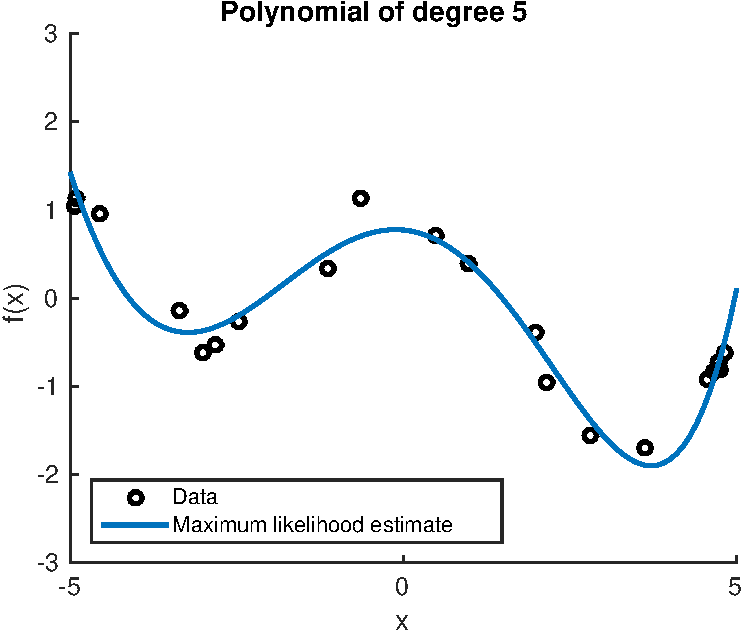
\includegraphics[width = 0.5\hsize]{./figures-crossval/polynomial5}
  \end{figure}
\vspace{-0.4cm}
\begin{itemize}
\item What we want: Find a curve that predicts well \emph{even for unseen inputs}
\item What we do: Minimise loss on \emph{training points}:
\begin{equation}
L(\vtheta) = \sum_n (f(\vx_n; \vtheta) - y_n)^2
\end{equation}
\end{itemize}
\end{frame}


\begin{frame}{Curve fitting}
We will investigate the consequences of
\begin{itemize}
\item choosing particular basis functions,
\item fitting to training points (\emph{overfitting}).
\end{itemize}

\pause
\vspace{0.3cm}

The two are related. Let's consider a sequence of linear regression models with polynomial basis functions:
\begin{equation}
\text{Model: } q \in {0, \dots, Q}: \vphi(x) = [1\,\,\dots\,\,x^q]\transpose
\end{equation} \pause

Two questions: As $q$ increases,
\begin{itemize}
\item what will happen to the \emph{training loss}?
\item how good do you think the predictions will be?
\end{itemize}
\end{frame}


\begin{frame}[t]{Basis functions}
\vspace{-0.2cm}
    \only<1>{\begin{figure}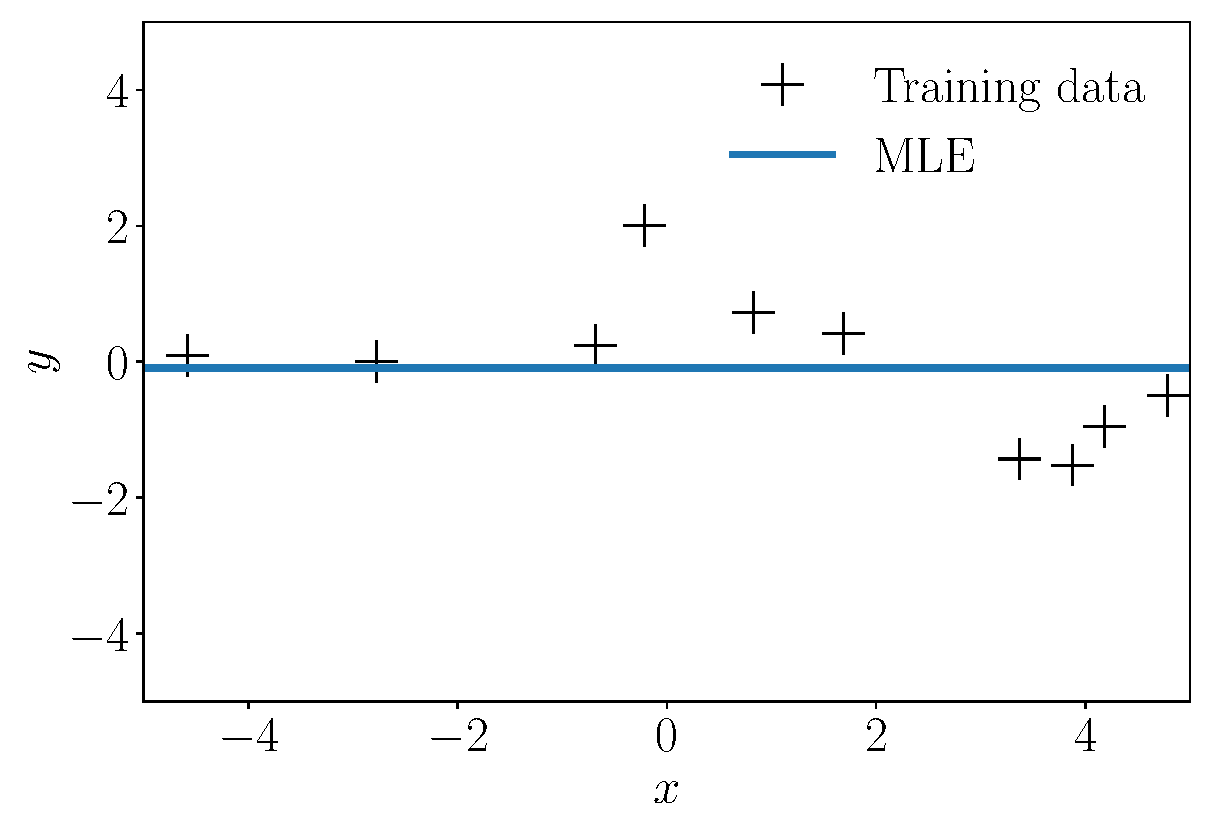
\includegraphics[width = 0.8\hsize]{./figures-crossval/demo_regression_mle_0.pdf}\end{figure}}
    \only<2>{\begin{figure}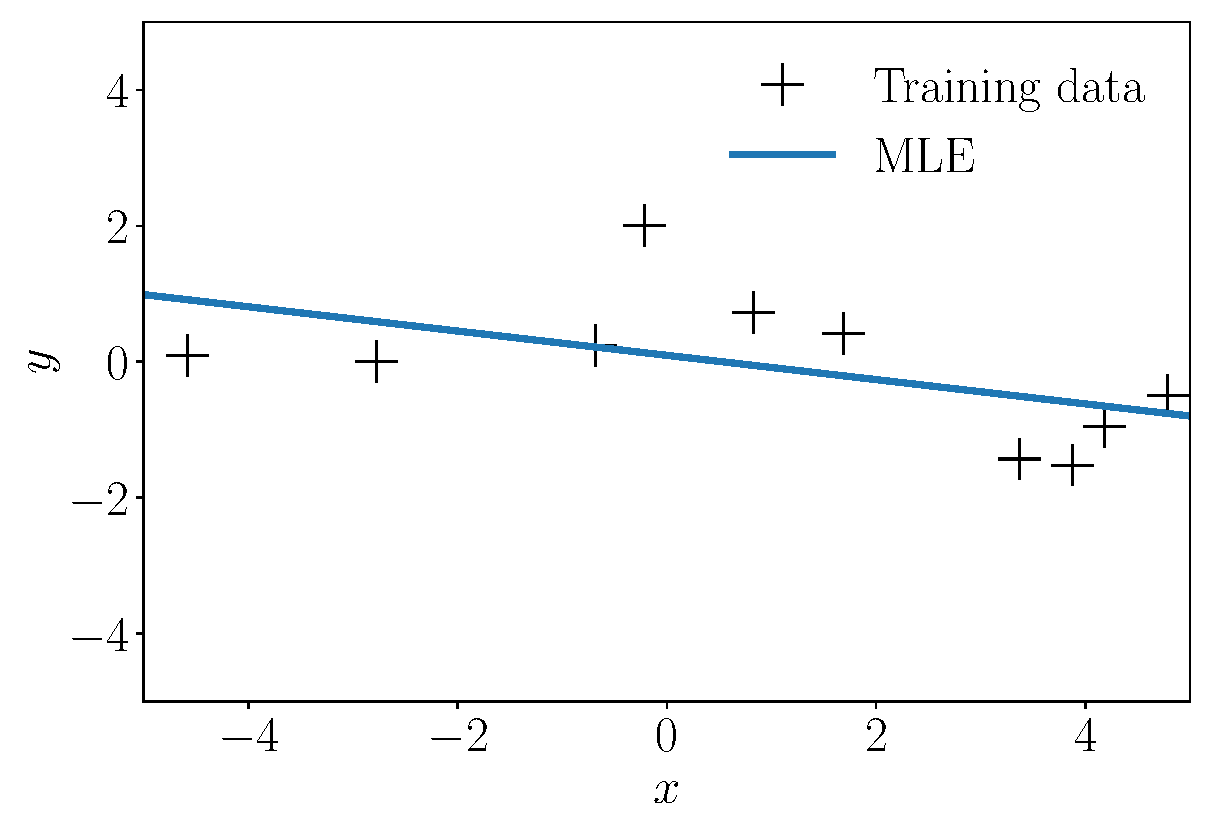
\includegraphics[width = 0.8\hsize]{./figures-crossval/demo_regression_mle_1.pdf}\end{figure}}
    \only<3>{\begin{figure}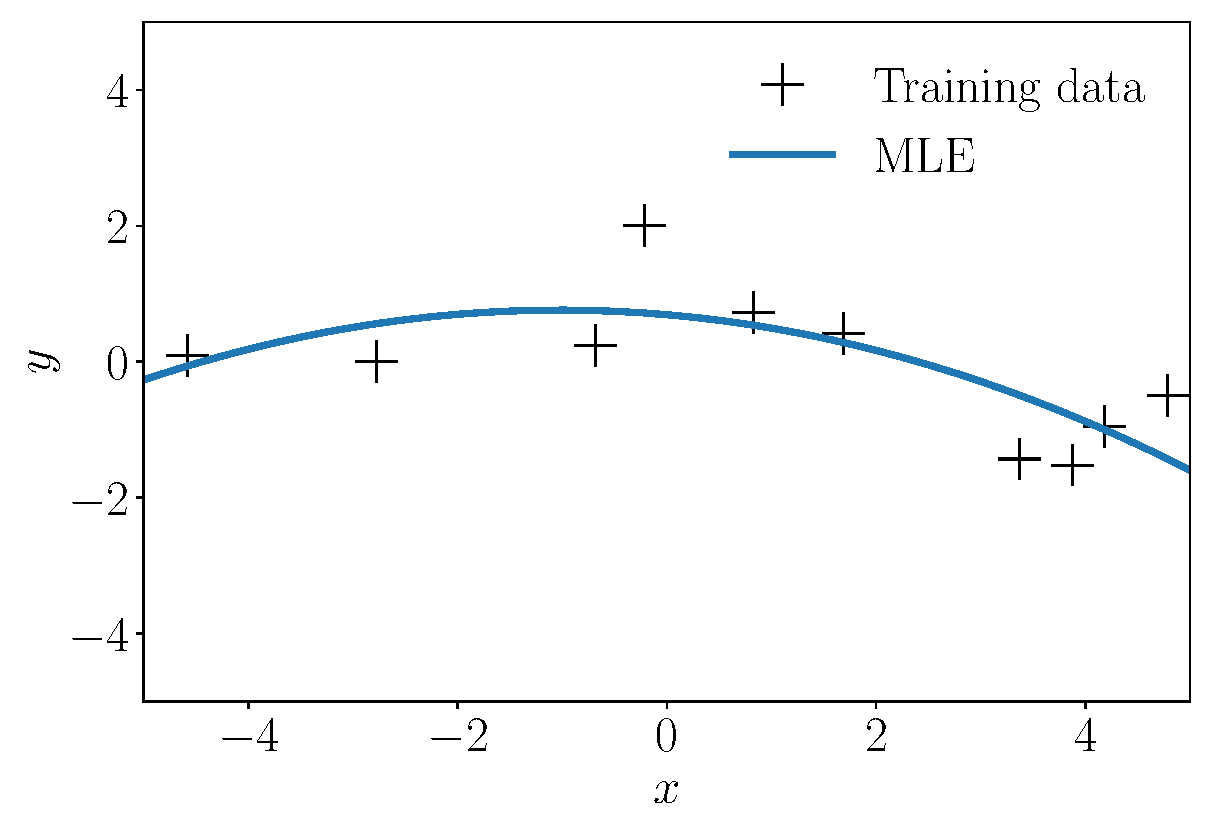
\includegraphics[width = 0.8\hsize]{./figures-crossval/demo_regression_mle_2.pdf}\end{figure}}
    \only<4>{\begin{figure}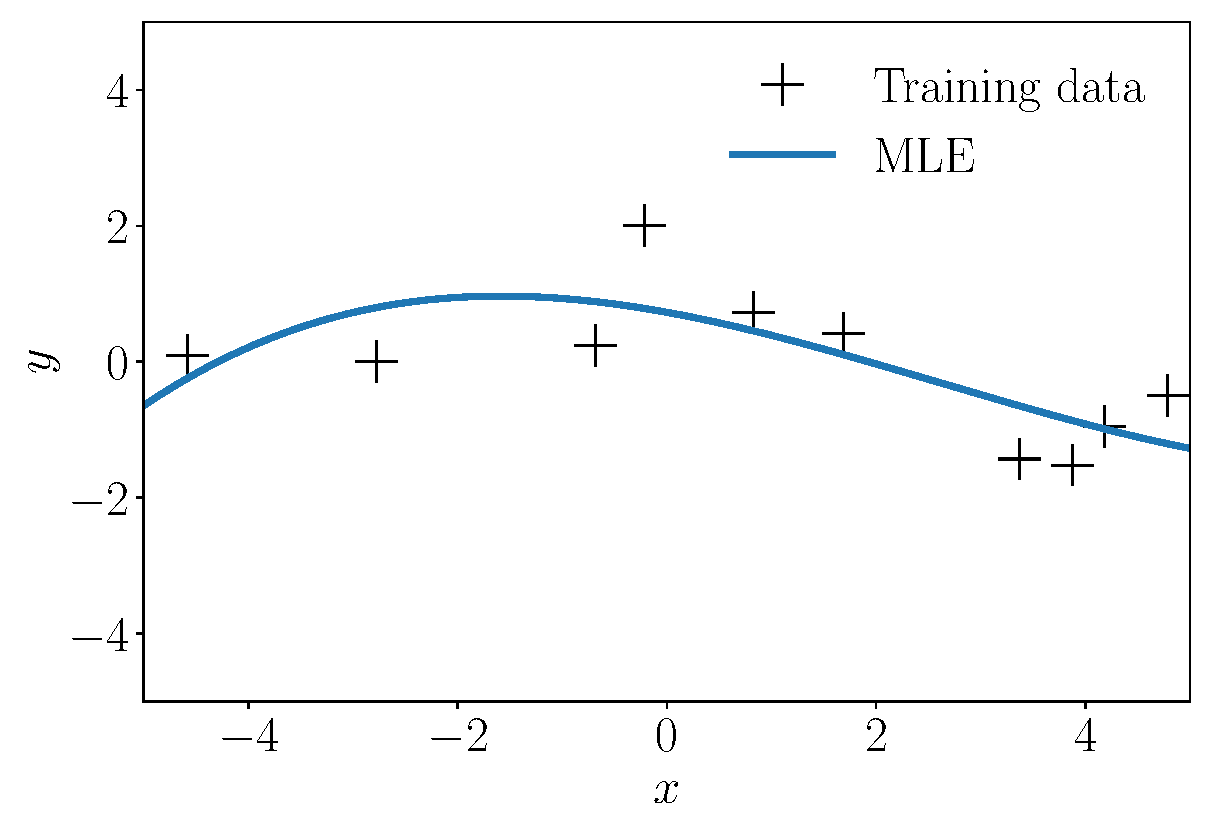
\includegraphics[width = 0.8\hsize]{./figures-crossval/demo_regression_mle_3.pdf}\end{figure}}
    \only<5>{\begin{figure}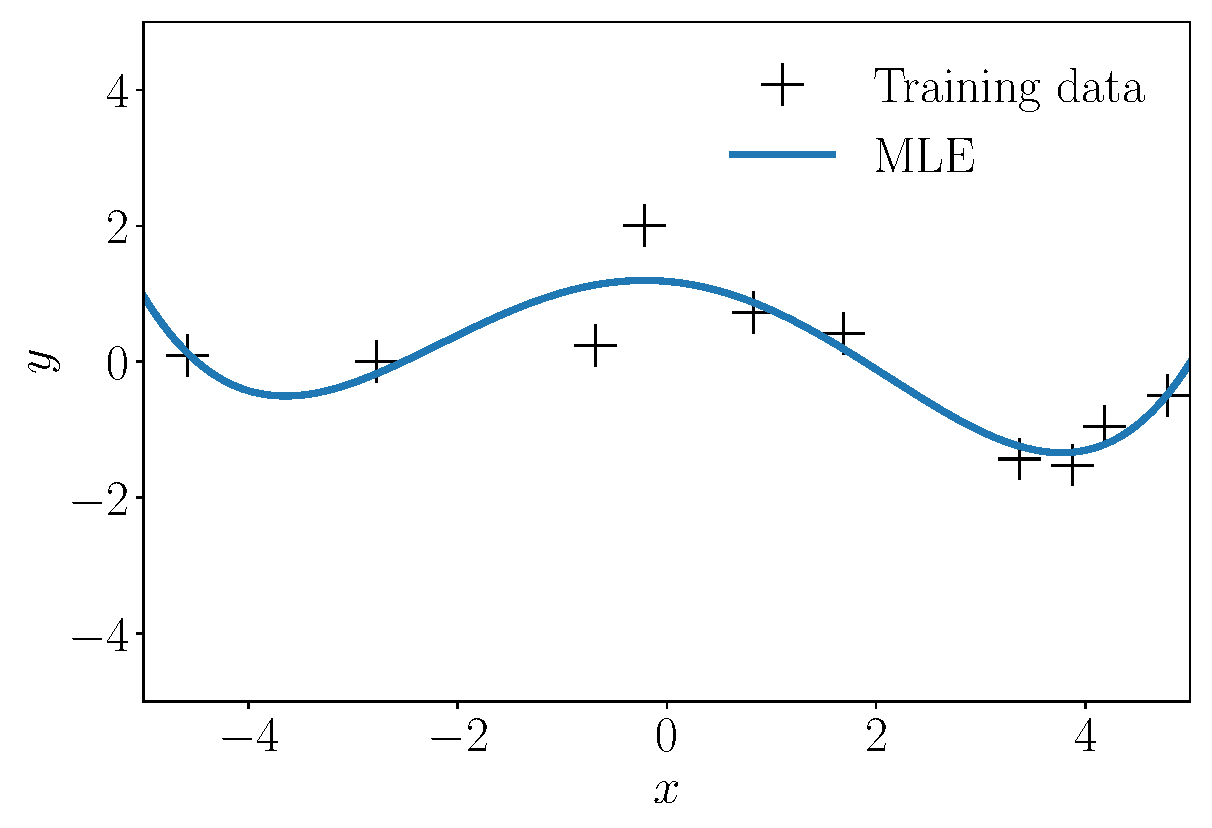
\includegraphics[width = 0.8\hsize]{./figures-crossval/demo_regression_mle_4.pdf}\end{figure}}
    \only<6>{\begin{figure}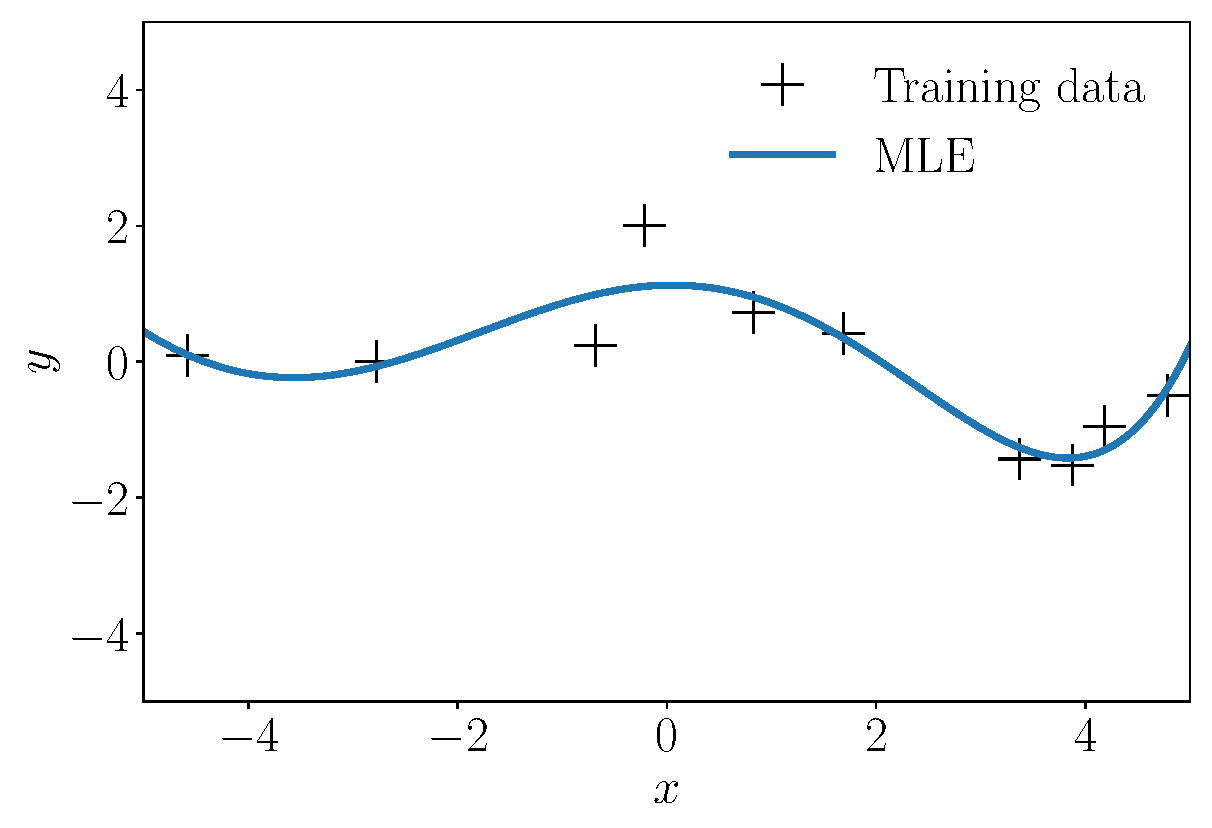
\includegraphics[width = 0.8\hsize]{./figures-crossval/demo_regression_mle_5.pdf}\end{figure}}
    \only<7>{\begin{figure}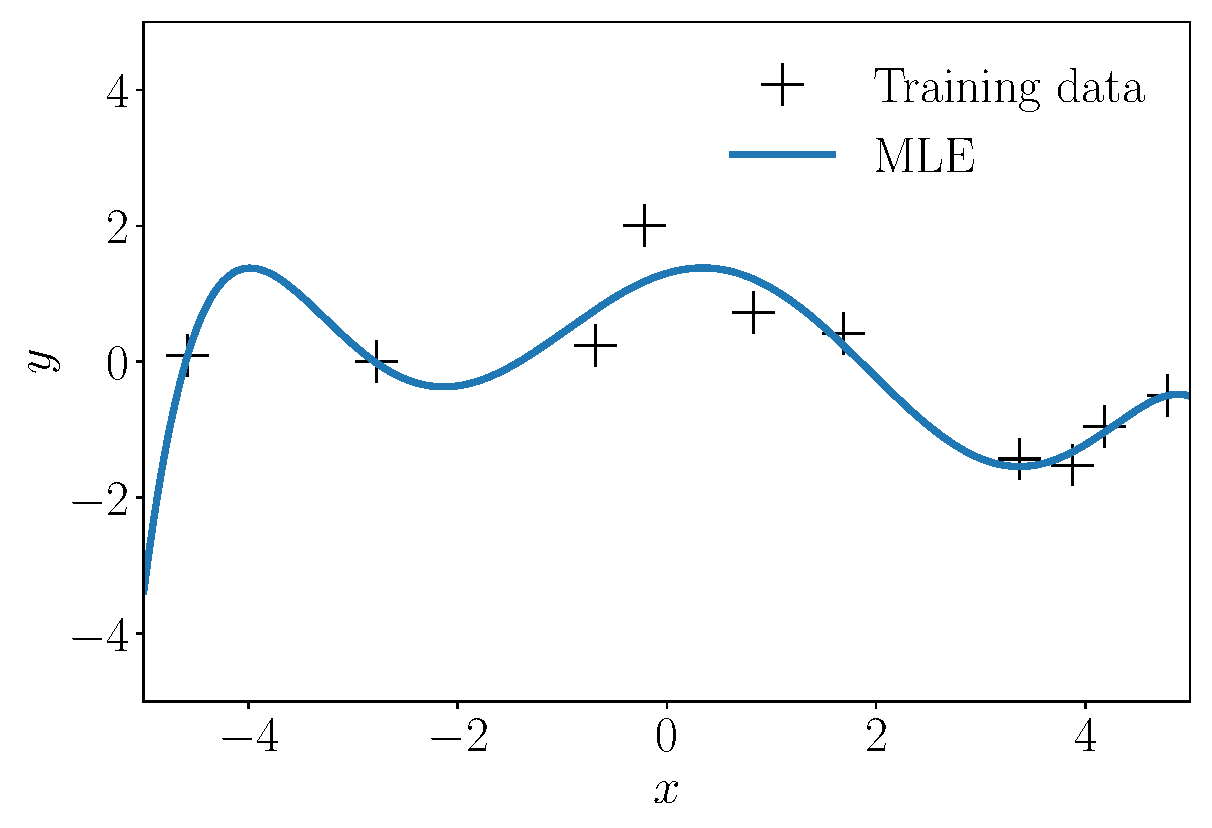
\includegraphics[width = 0.8\hsize]{./figures-crossval/demo_regression_mle_6.pdf}\end{figure}}
    \only<8>{\begin{figure}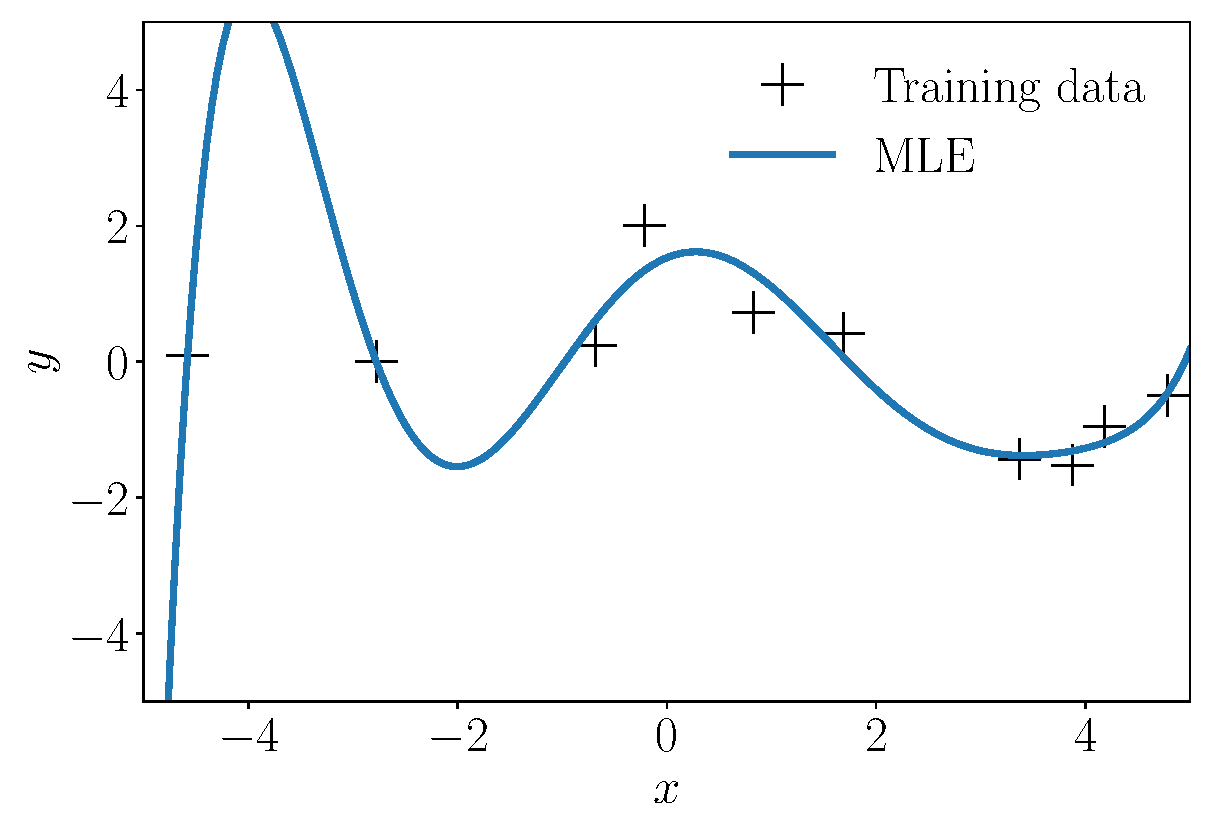
\includegraphics[width = 0.8\hsize]{./figures-crossval/demo_regression_mle_7.pdf}\end{figure}}
    \only<9>{\begin{figure}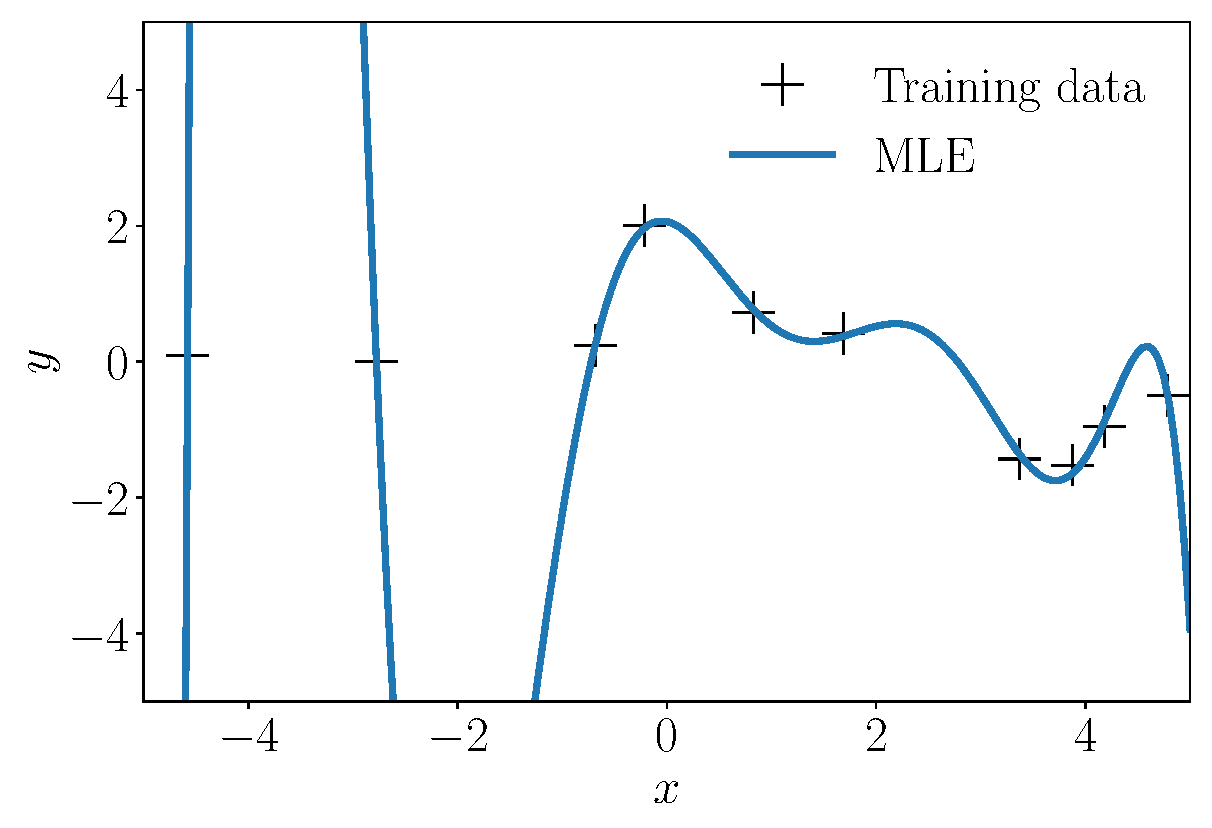
\includegraphics[width = 0.8\hsize]{./figures-crossval/demo_regression_mle_8.pdf}\end{figure}}
    \only<10>{\begin{figure}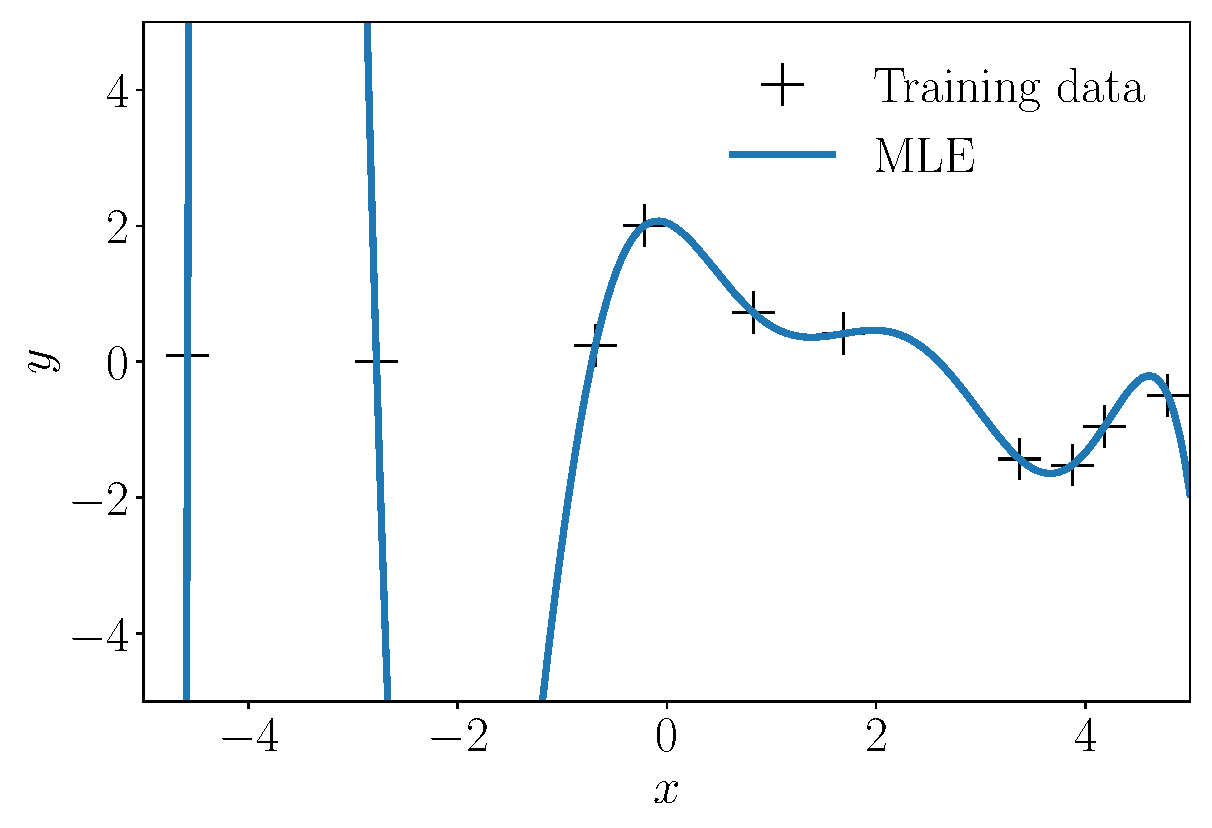
\includegraphics[width = 0.8\hsize]{./figures-crossval/demo_regression_mle_9.pdf}\end{figure}}
    \only<11>{\begin{figure}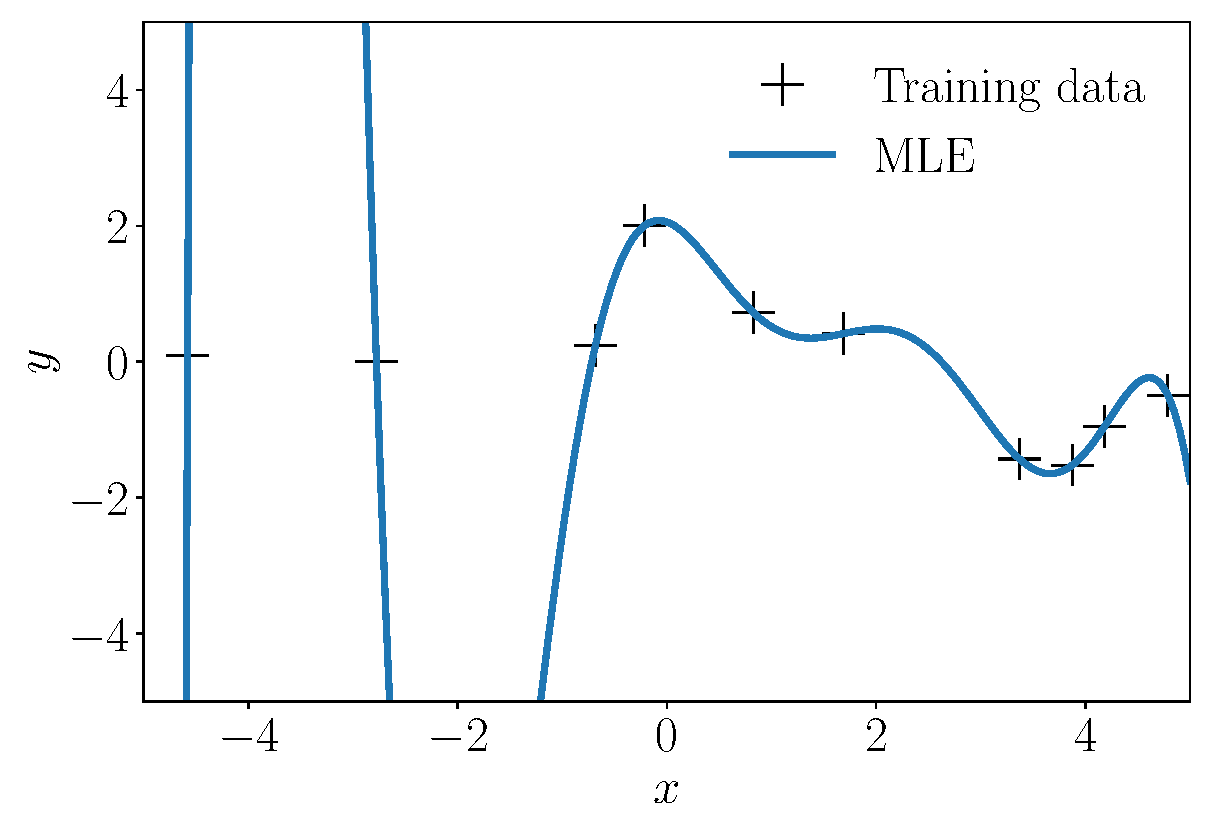
\includegraphics[width = 0.8\hsize]{./figures-crossval/demo_regression_mle_10.pdf}\end{figure}}
\only<1>{
\begin{equation}
\vphi(x) = [1]\transpose
\end{equation}
}
\only<2>{
\begin{equation}
\vphi(x) = [1\,\, x]\transpose
\end{equation}
}
\only<3>{
\begin{equation}
\vphi(x) = [1\,\, x\,\, x^2]\transpose
\end{equation}
}
\only<4>{
\begin{equation}
\vphi(x) = [1\,\, x\,\, x^2\,\, x^3]\transpose
\end{equation}
}
\only<4->{
\begin{equation}
\vphi(x) = [1\,\, x\,\, x^2\,\, x^3, \dots]\transpose
\end{equation}
}
\end{frame}


\begin{frame}{Training loss}
Q: How does the training loss change as $M$ increases?
\begin{gather}
L_M(\vtheta) = \sum_n (f_M(\vx_n; \vtheta) - y_n)^2\,, \qquad\quad
f_M(\vx_n; \vtheta) = \sum_{m=0}^M x^m \theta_m
\end{gather}
\pause
\begin{itemize}
\item For two models with $M_1 \leq M_2$, model $M_2$ can represent \textit{all} functions that $M_1$ can, and more. \pause
\item Remember: Closed-form optimisation finds the \emph{exact} minimum. \pause
\end{itemize}
\begin{equation}
\implies \min_{\vtheta} L_{M_2}(\vtheta) \leq \min_{\vtheta} L_{M_1}(\vtheta)
\end{equation} \pause
\begin{center}
Training loss always gets smaller as we add basis functions. \pause \\
{\Large But what about the predictions?}
\end{center}
\end{frame}



\begin{frame}{Train/Test Split}
Some machine learning ``good practice''...
\begin{center}
\large How can we tell \\ how well a model will predict on \emph{unseen} data?
\end{center} \pause
You probably already know the procedure: \pause
\begin{itemize}
\item Split all data into a \emph{training set} and \emph{test set}. \pause
\item Only train on training set, and \emph{measure} loss on the test set:
\begin{gather}
\vtheta^* = \argmin_{\vtheta} L(\vtheta) \\
L_{\text{test}} = \frac{1}{N_{\text{test}}}\sum_{n=1}^{N_{\text{test}}}\ell(f(x_n; \vtheta^*), y_n) \,, \qquad (x_n, y_n) \in \mathcal{S}_{\text{test}}
\end{gather} \pause
\vspace{-0.4cm}
\end{itemize}
\begin{center}
\Large \emph{Why does this work?}
\end{center}
\end{frame}



\begin{frame}{Generalisation performance}
Our question is not precise enough: \pause
\begin{itemize}
\item How will our predictions on unseen data affect us? \pause
\item But what is unseen data? \pause
\item What assumptions underlie this reasoning? \pause
\end{itemize}

\vspace{0.4cm}

Let's make the question precise by:
\begin{itemize}
\item Specifying one way for how we will use our predictions.
\item Using the assumptions from lecture 1.
\end{itemize}

\end{frame}


\begin{frame}{Predictions and Losses}
\begin{itemize}
\item Imagine deploying a ML system in production \\
(predicting ad value, engine fuel control system) \pause
\item If widely deployed, you will make \emph{many} predictions \pause
\item We incur a loss for error in the predictions \pause
\item Let's measure the loss per prediction.
\begin{align}
L_{\text{deploy}} = \frac{1}{N_{\text{deploy}}} \sum_{n=1}^{N_{\text{deploy}}} \ell(f(x_n, \vtheta^*), y_n)
\end{align} \pause
\item Many predictions: $N_{\text{deploy}} \to \infty$ \pause
\item Does it even make sense? Is this quantity even well-defined?
\end{itemize}


\end{frame}




\begin{frame}{Statistical View on the World}
\begin{myblock}{Data Generating Process}
We assume that the data we observe is the outcome of some random process. Each observation is one random variable. In this course, probabilities of the data generating process are denoted with $\mathbb P(\cdot)$, and which has distribution $\pi(\cdot)$.
\end{myblock} \pause

Example:
\begin{itemize}
\item We observe a dataset of 3 values $\{x_n\}_{n=1}^3$.
\item This has density $\pi_{X_1,X_2,X_3}(x_1, x_2, x_3)$.
\end{itemize}

\end{frame}


\begin{frame}{Independent Identically Distributed}
\begin{myblock}{Independent Identically Distributed (iid) Assumption}
Often, we assume that random variables in a dataset are independent and identically distributed, which means that each random variable has the same distribution. Groups of RVs can also be iid.
\end{myblock} \pause

Examples:
\begin{align*}
\pi_{X_1,X_2,X_3}(x_1, x_2, x_3) &= \prod_{n=1}^3\pi(x_n) \\
\pi_{X_1,Y_1,X_2,Y_2,\dots}(x_1, y_1, x_2, y_2, \dots) &= \pi_{X,Y}(\vx,\vy) && \vx,\vy\in\Reals^N \\
&= \prod_{n=1}^N \pi(x_n, y_n)
\end{align*}
\end{frame}


\begin{frame}{Expected Loss}
\begin{itemize}
\item $x_n, y_n \overset{\mathrm{iid}}{\sim} \pi$ \pause
\item $N_{\text{deploy}} \to \infty$ \pause
\item So intuitively
\begin{align}
L_{\text{deploy}} &= \frac{1}{N_{\text{deploy}}} \sum_{n=1}^{N_{\text{deploy}}}\ell(f(x_n, \vtheta^*), y_n) \\
&\approx \Exp{\pi(x, y)}{\ell\left(f(x, \vtheta^*), y\right)}
\end{align} \pause
\vspace{-0.4cm}
\item Finally, a well-defined quantity \pause
\item Only meaningful because of the iid assumption! \pause
\item Let's use a \emph{theorem} to prove this.
\end{itemize}
\end{frame}


\begin{frame}{Weak Law of Large Numbers} 
In what sense does the $\approx$ hold? \pause \\

\vspace{0.3cm}

Weak Law of Large Numbers:
\begin{itemize}
\item For a sequence of iid RVs $X_1, X_2, X_3, \dots, X_N$ \pause
\item with mean $\mu = \Exp{}{X}$ \pause
\item we can define a new RV $\overline{X}_N\ = \frac{1}{N}\sum_{n=1}^N X_n$ \pause
\item for which will hold:
\begin{align}
\lim_{N\to\infty}\mathbb P\left(|\overline X_n - \mu| < \epsilon\right) = 1
\end{align}
\end{itemize}
\end{frame}




\begin{frame}{Expected Loss}
Deploy loss converging to expected loss:
\begin{itemize}
\item $x_n, y_n \overset{\mathrm{iid}}{\sim} \pi_{X,Y} \implies \ell_n = \ell(f(x_n), y_n))$ is a RV, with density $\pi(\ell_n)$ \pause
\item $L_{\text{deploy}}^{N_{\text{deploy}}} = \frac{1}{N_{\text{deploy}}} \sum_{n=1}^{N_{\text{deploy}}} \ell_n $ \pause
\item By Weak LLN
\begin{align}
\lim_{N_{\text{deploy} \to \infty}} \mathbb P(|L_{\text{deploy}} - \mu| < \epsilon) = 1
\end{align} \pause
\item With $\mu = \Exp{\pi(\ell)}{\ell} = \Exp{\pi(x, y)}{\ell\left(f(x, \vtheta^*), y\right)}$ by LOTUS
\end{itemize}
\end{frame}


\begin{frame}{Monte Carlo Estimate of the Expected Loss}
\begin{itemize}
\item We now know that the deploy loss is well-defined \pause
\item But, we can't compute it: don't know $\pi_{X,Y}$ \pause
\item Can we estimate it? \pause
\item Previous process in reverse $\implies$ \emph{Monte Carlo} estimation
\end{itemize}
% By exactly the same argument, we can see that for the test set loss
% \begin{align}
% L_{\text{test}} = \frac{1}{N_{\text{test}}}\sum_{n=1}^{N_{\text{test}}}\ell(f(x_n; \vtheta^*), y_n) \,, \qquad (x_n, y_n) \in \mathcal{S}_{\text{test}}
% \end{align}
% where $x_n, y_n \overset{\mathrm{iid}}{\sim} \pi_{X,Y}$, we have
% \begin{align}
% \lim_{N_{\text{test} \to \infty}} \mathbb P(|L_{\text{test}} - \mu| < \epsilon) = 1 \,,
% \end{align}
% with $\mu = \Exp{\pi(x, y)}{\ell\left(f(x, \vtheta^*), y\right)}$. \pause

% \vspace{0.3cm}
% \begin{itemize}
% \item Test loss is an estimate of the expected loss, which is accurate if $N_{\text{test}}$ is large enough.
% \item 
% \end{itemize}
\end{frame}


\begin{frame}{Monte Carlo Estimation}
Want to find a difficult expectation / integral:
\begin{align}
I = \int p_X(x) f(x) \calcd x =  \Exp{p_X(X)}{f(X)}
\end{align} \pause

Use estimator
\begin{align}
\hat I = \frac{1}{N}\sum_{n=1}^N f(x_n) && x_n \overset{\mathrm{iid}}{\sim} p_X
\end{align} \pause

By considering it as a sum of independent RVs:
\begin{itemize}
\item Can show it to be \emph{unbiased}, i.e.~$\Exp{p(x_1, x_2, \dots)}{\hat I} = I$ (board).
\item Can show the variance reduces as $c / N$ (board).
\item Weak LLN implies $\lim_{N\to\infty} P(|\hat I - I| < \epsilon) = 1$ (relies on unbiasedness!)
\end{itemize}
\end{frame}



\begin{frame}{Overfitting}
Can use test loss estimator to \emph{evaluate} various models:
  \begin{figure}
    \centering
    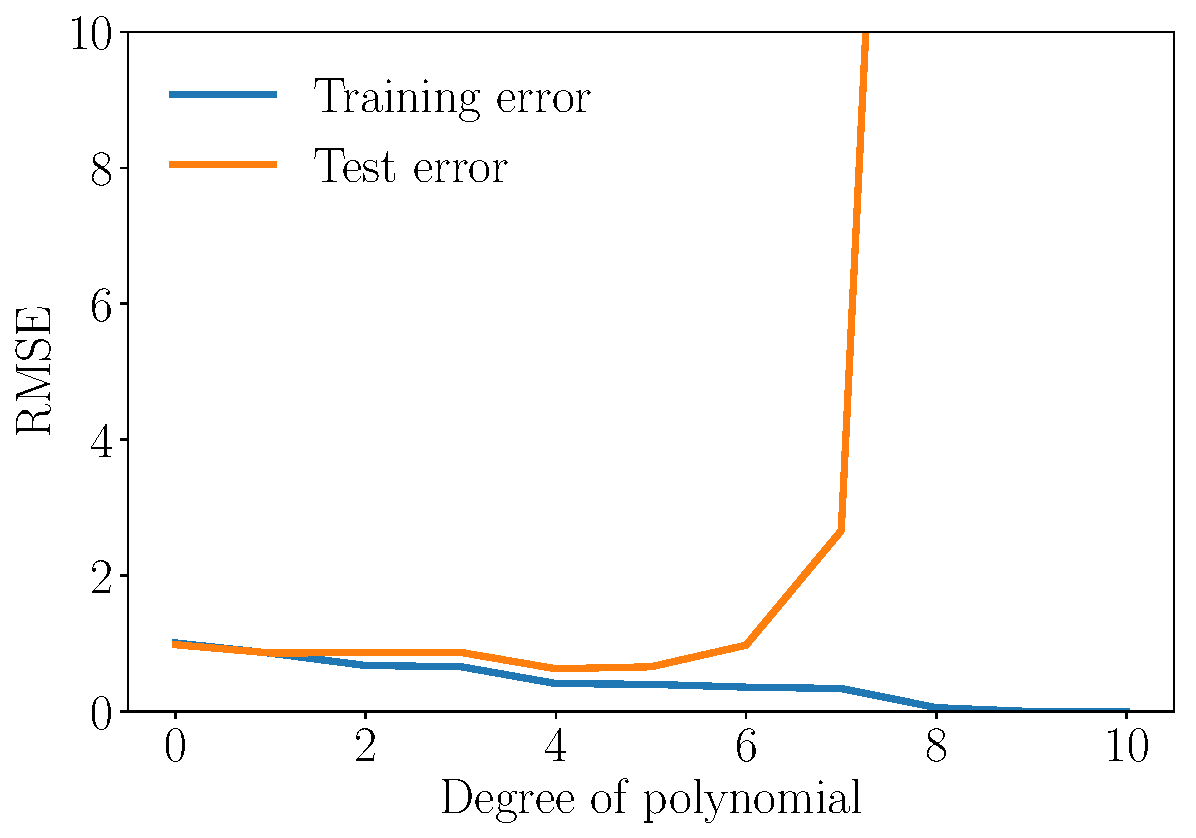
\includegraphics[width = 0.5\hsize]{./figures-crossval/demo_regression_training_test_RMSE}
  \end{figure} \pause
\begin{itemize}
\item We indeed see that training error continuously decreases.
\item Test error only decreases with train error up to a point!
\item When test error starts increasing $\implies$ overfitting.
\end{itemize}
\end{frame}









\begin{frame}{Model selection}
% Once we made our choices for our model (e.g.~degree of polynomial), we know how to find parameters. \pause
We can prevent overfitting by choosing a model which isn't too flexible.

\vspace{0.4cm}

\begin{center}
{\Large Q: How do we decide which model to use?} \\ \pause
{$\implies$ \emph{model selection}}
\end{center} \pause

\end{frame}


\begin{frame}{Summary}
\begin{itemize}
\item Overfitting
\item Assumptions behind test sets (many predictions + iid data generation)
\item Law of Large Numbers (skill)
\item Monte Carlo estimation (skill)
\end{itemize}

% \vspace{0.3cm} \pause
% Next time:
% \begin{itmeize}
% \item Prove Weak LLN
% \item Prove bounds of form
% \begin{align}
% \mathbb P(\mathrm{ExpRisk} > L_\epsilon) < \delta
% \end{align}
% \end{itemize}
\end{frame}












\end{document}
%%% Local Variables: 
%%% mode: latex
%%% TeX-master: t
%%% End: 
